\documentclass[8pt]{beamer}

% Beamer style
%\usetheme[secheader]{Madrid}
% \usetheme{CambridgeUS}
\useoutertheme{infolines}
\usecolortheme[rgb={0.65,0.15,0.25}]{structure}
% \usefonttheme[onlymath]{serif}
\beamertemplatenavigationsymbolsempty
%\AtBeginSubsection

% Packages
%\usepackage[french]{babel}
\usepackage[latin1]{inputenc}
\usepackage{color}
% \usepackage[dvipsnames]{xcolor}
\usepackage{xspace}
\usepackage{dsfont, stmaryrd}
\usepackage{amsmath, amsfonts, amssymb, stmaryrd, mathabx}
\usepackage{epsfig}
\usepackage{tikz}
\usepackage{url}
% \usepackage{ulem}
\usepackage{/home/robin/LATEX/Biblio/astats}
%\usepackage[all]{xy}
\usepackage{graphicx}

% Maths
% \newtheorem{theorem}{Theorem}
% \newtheorem{definition}{Definition}
\newtheorem{proposition}{Proposition}
% \newtheorem{assumption}{Assumption}
% \newtheorem{algorithm}{Algorithm}
% \newtheorem{lemma}{Lemma}
% \newtheorem{remark}{Remark}
% \newtheorem{exercise}{Exercise}
% \newcommand{\propname}{Prop.}
% \newcommand{\proof}{\noindent{\sl Proof:}\quad}
% \newcommand{\eproof}{$\blacksquare$}

% \setcounter{secnumdepth}{3}
% \setcounter{tocdepth}{3}
\newcommand{\pref}[1]{\ref{#1} p.\pageref{#1}}
\newcommand{\qref}[1]{\eqref{#1} p.\pageref{#1}}

% Colors : http://latexcolor.com/
\definecolor{darkred}{rgb}{0.65,0.15,0.25}
\definecolor{darkgreen}{rgb}{0,0.4,0}
\definecolor{darkred}{rgb}{0.65,0.15,0.25}
\definecolor{amethyst}{rgb}{0.6, 0.4, 0.8}
\definecolor{asparagus}{rgb}{0.53, 0.66, 0.42}
\definecolor{applegreen}{rgb}{0.55, 0.71, 0.0}
\definecolor{awesome}{rgb}{1.0, 0.13, 0.32}
\definecolor{blue-green}{rgb}{0.0, 0.87, 0.87}
\definecolor{red-ggplot}{rgb}{0.52, 0.25, 0.23}
\definecolor{green-ggplot}{rgb}{0.42, 0.58, 0.00}
\definecolor{purple-ggplot}{rgb}{0.34, 0.21, 0.44}
\definecolor{blue-ggplot}{rgb}{0.00, 0.49, 0.51}

% Commands
\newcommand{\backupbegin}{
   \newcounter{finalframe}
   \setcounter{finalframe}{\value{framenumber}}
}
\newcommand{\backupend}{
   \setcounter{framenumber}{\value{finalframe}}
}
\newcommand{\emphase}[1]{\textcolor{darkred}{#1}}
\newcommand{\comment}[1]{\textcolor{gray}{#1}}
\newcommand{\paragraph}[1]{\textcolor{darkred}{#1}}
\newcommand{\refer}[1]{{\small{\textcolor{gray}{{\cite{#1}}}}}}
\newcommand{\Refer}[1]{{\small{\textcolor{gray}{{[#1]}}}}}
\newcommand{\goto}[1]{{\small{\textcolor{blue}{[\#\ref{#1}]}}}}
\renewcommand{\newblock}{}

\newcommand{\tabequation}[1]{{\medskip \centerline{#1} \medskip}}
% \renewcommand{\binom}[2]{{\left(\begin{array}{c} #1 \\ #2 \end{array}\right)}}

% Variables 
\newcommand{\Abf}{{\bf A}}
\newcommand{\Beta}{\text{B}}
\newcommand{\Bcal}{\mathcal{B}}
\newcommand{\Bias}{\xspace\mathbb B}
\newcommand{\Cor}{{\mathbb C}\text{or}}
\newcommand{\Cov}{{\mathbb C}\text{ov}}
\newcommand{\cl}{\text{\it c}\ell}
\newcommand{\Ccal}{\mathcal{C}}
\newcommand{\cst}{\text{cst}}
\newcommand{\Dcal}{\mathcal{D}}
\newcommand{\Ecal}{\mathcal{E}}
\newcommand{\Esp}{\xspace\mathbb E}
\newcommand{\Espt}{\widetilde{\Esp}}
\newcommand{\Covt}{\widetilde{\Cov}}
\newcommand{\Ibb}{\mathbb I}
\newcommand{\Fcal}{\mathcal{F}}
\newcommand{\Gcal}{\mathcal{G}}
\newcommand{\Gam}{\mathcal{G}\text{am}}
\newcommand{\Hcal}{\mathcal{H}}
\newcommand{\Jcal}{\mathcal{J}}
\newcommand{\Lcal}{\mathcal{L}}
\newcommand{\Mt}{\widetilde{M}}
\newcommand{\mt}{\widetilde{m}}
\newcommand{\Nbb}{\mathbb{N}}
\newcommand{\Mcal}{\mathcal{M}}
\newcommand{\Ncal}{\mathcal{N}}
\newcommand{\Ocal}{\mathcal{O}}
\newcommand{\pt}{\widetilde{p}}
\newcommand{\Pt}{\widetilde{P}}
\newcommand{\Pbb}{\mathbb{P}}
\newcommand{\Pcal}{\mathcal{P}}
\newcommand{\Qcal}{\mathcal{Q}}
\newcommand{\qt}{\widetilde{q}}
\newcommand{\Rbb}{\mathbb{R}}
\newcommand{\Sbb}{\mathbb{S}}
\newcommand{\Scal}{\mathcal{S}}
\newcommand{\st}{\widetilde{s}}
\newcommand{\St}{\widetilde{S}}
\newcommand{\Tcal}{\mathcal{T}}
\newcommand{\todo}{\textcolor{red}{TO DO}}
\newcommand{\Ucal}{\mathcal{U}}
\newcommand{\Un}{\math{1}}
\newcommand{\Vcal}{\mathcal{V}}
\newcommand{\Var}{\mathbb V}
\newcommand{\Vart}{\widetilde{\Var}}
\newcommand{\Zcal}{\mathcal{Z}}

% Symboles & notations
\newcommand\independent{\protect\mathpalette{\protect\independenT}{\perp}}\def\independenT#1#2{\mathrel{\rlap{$#1#2$}\mkern2mu{#1#2}}} 
\renewcommand{\d}{\text{\xspace d}}
\newcommand{\gv}{\mid}
\newcommand{\ggv}{\, \| \, }
% \newcommand{\diag}{\text{diag}}
\newcommand{\card}[1]{\text{card}\left(#1\right)}
\newcommand{\trace}[1]{\text{tr}\left(#1\right)}
\newcommand{\matr}[1]{\boldsymbol{#1}}
\newcommand{\matrbf}[1]{\mathbf{#1}}
\newcommand{\vect}[1]{\matr{#1}} %% un peu inutile
\newcommand{\vectbf}[1]{\matrbf{#1}} %% un peu inutile
\newcommand{\trans}{\intercal}
\newcommand{\transpose}[1]{\matr{#1}^\trans}
\newcommand{\crossprod}[2]{\transpose{#1} \matr{#2}}
\newcommand{\tcrossprod}[2]{\matr{#1} \transpose{#2}}
\newcommand{\matprod}[2]{\matr{#1} \matr{#2}}
\DeclareMathOperator*{\argmin}{arg\,min}
\DeclareMathOperator*{\argmax}{arg\,max}
\DeclareMathOperator{\sign}{sign}
\DeclareMathOperator{\tr}{tr}
\newcommand{\ra}{\emphase{$\rightarrow$} \xspace}

% Hadamard, Kronecker and vec operators
\DeclareMathOperator{\Diag}{Diag} % matrix diagonal
\DeclareMathOperator{\diag}{diag} % vector diagonal
\DeclareMathOperator{\mtov}{vec} % matrix to vector
\newcommand{\kro}{\otimes} % Kronecker product
\newcommand{\had}{\odot}   % Hadamard product

% TikZ
\newcommand{\nodesize}{2em}
\newcommand{\edgeunit}{2.5*\nodesize}
\newcommand{\edgewidth}{1pt}
\tikzstyle{node}=[draw, circle, fill=black, minimum width=.75\nodesize, inner sep=0]
\tikzstyle{square}=[rectangle, draw]
\tikzstyle{param}=[draw, rectangle, fill=gray!50, minimum width=\nodesize, minimum height=\nodesize, inner sep=0]
\tikzstyle{hidden}=[draw, circle, fill=gray!50, minimum width=\nodesize, inner sep=0]
\tikzstyle{hiddenred}=[draw, circle, color=red, fill=gray!50, minimum width=\nodesize, inner sep=0]
\tikzstyle{observed}=[draw, circle, minimum width=\nodesize, inner sep=0]
\tikzstyle{observedred}=[draw, circle, minimum width=\nodesize, color=red, inner sep=0]
\tikzstyle{eliminated}=[draw, circle, minimum width=\nodesize, color=gray!50, inner sep=0]
\tikzstyle{empty}=[draw, circle, minimum width=\nodesize, color=white, inner sep=0]
\tikzstyle{blank}=[color=white]
\tikzstyle{nocircle}=[minimum width=\nodesize, inner sep=0]

\tikzstyle{edge}=[-, line width=\edgewidth]
\tikzstyle{edgebendleft}=[-, >=latex, line width=\edgewidth, bend left]
\tikzstyle{edgebendright}=[-, >=latex, line width=\edgewidth, bend right]
\tikzstyle{lightedge}=[-, line width=\edgewidth, color=gray!50]
\tikzstyle{lightedgebendleft}=[-, >=latex, line width=\edgewidth, bend left, color=gray!50]
\tikzstyle{lightedgebendright}=[-, >=latex, line width=\edgewidth, bend right, color=gray!50]
\tikzstyle{edgered}=[-, line width=\edgewidth, color=red]
\tikzstyle{edgebendleftred}=[-, >=latex, line width=\edgewidth, bend left, color=red]
\tikzstyle{edgebendrightred}=[-, >=latex, line width=\edgewidth, bend right, color=red]

\tikzstyle{arrow}=[->, >=latex, line width=\edgewidth]
\tikzstyle{arrowbendleft}=[->, >=latex, line width=\edgewidth, bend left]
\tikzstyle{arrowbendright}=[->, >=latex, line width=\edgewidth, bend right]
\tikzstyle{arrowred}=[->, >=latex, line width=\edgewidth, color=red]
\tikzstyle{arrowbendleftred}=[->, >=latex, line width=\edgewidth, bend left, color=red]
\tikzstyle{arrowbendrightred}=[->, >=latex, line width=\edgewidth, bend right, color=red]
\tikzstyle{arrowblue}=[->, >=latex, line width=\edgewidth, color=blue]
\tikzstyle{dashedarrow}=[->, >=latex, dashed, line width=\edgewidth]
\tikzstyle{dashededge}=[-, >=latex, dashed, line width=\edgewidth]
\tikzstyle{dashededgebendleft}=[-, >=latex, dashed, line width=\edgewidth, bend left]
\tikzstyle{lightarrow}=[->, >=latex, line width=\edgewidth, color=gray!50]


% Directory
\newcommand{\figcp}{/home/robin/RECHERCHE/RUPTURES/EXPOSES/FIGURES}
\newcommand{\figgen}{/home/robin/RECHERCHE/GENOME/EXPOSES/FIGURES}
\newcommand{\figexp}{/home/robin/RECHERCHE/EXPRESSION/EXPOSES/FIGURES}
\newcommand{\figeco}{/home/robin/RECHERCHE/ECOLOGIE/EXPOSES/FIGURES}
\newcommand{\figfdr}{/home/robin/RECHERCHE/COMPMULT/EXPOSES/FIGURES}
\newcommand{\figmhs}{/home/robin/ENSEIGN/CoursAgro/MOD-GRAPH/Figures}
\newcommand{\figbayes}{/home/robin/RECHERCHE/BAYES/EXPOSES/FIGURES}

%====================================================================
%====================================================================

%====================================================================
%====================================================================
\begin{document}
%====================================================================
%====================================================================

%====================================================================
\title[Latent variables in genomics]{A partial history of latent variable models in genomics}

\author[S. Robin]{S. Robin + many others}

\institute[]{LPSM, Sorbonne universit�}

\date[SMPGD, Paris, Feb. 2024]{Statistical Methods for Post Genomic Data, 2024}

%====================================================================
%====================================================================
\maketitle

%====================================================================
%====================================================================
\section*{Introduction}
%====================================================================
\frame{\frametitle{Introduction}

  \paragraph{Latent variable model.} Model involving unobserved (= 'latent' = 'hidden' = \dots) variables.
  
  \bigskip \bigskip \pause
  \paragraph{Use for modelling.} Account for
  \begin{itemize}
  \item missing information (e.g. classification)
  \item dependency structure
  \item over-dispersion, \dots
  \end{itemize}
  
  \bigskip \bigskip \pause
  \paragraph{Notations.}
  $$
  \emphase{Y =} \text{ observed variables (data)}, \qquad
  \emphase{\theta =} \text{ model parameters}, \qquad
  \emphase{Z =} \text{ latent variables}
  $$
%   \begin{description}
%   \item[$Y = $] observed variables (data)
%   \item[$\theta =$] model parameters
%   \item[$Z = $] latent variables
%   \end{description}
  
  \bigskip \bigskip \pause
  \paragraph{Parameters $\neq$ latent variables.}
  \begin{itemize}
    \item $\theta$ can be fixed or random (e.g. frequentist vs Bayesian)
    \item $Z$ is random, $\simeq$ same dimension as $Y$
  \end{itemize}

}

%====================================================================
\frame{\frametitle{Inference}

  \paragraph{Intractable likelihood.} 
  $$
  \log p_\theta (Y) = \log \int p_\theta(Y, z) \d z 
  $$
  
  \bigskip \pause
  \paragraph{Popular approach.} Use the decomposition \refer{DLR77} 
  \begin{align*}
    \log p_\theta (Y) 
%     & =  \Esp_\theta[\log p_\theta(Y, Z) \mid Y] - \Esp_\theta[\log p_\theta(Z \mid Y) \mid Y] \\ 
    & =  \Esp_\theta[\emphase{\log p_\theta(Y, Z)} \mid Y] + \underset{\text{entropy}}{\underbrace{\Hcal_\theta(Z \mid Y)}}
  \end{align*}
  \pause
  and apply the iterative expectation-maximization (EM) algorithm:
  $$
  \theta^{(h+1)} = \underset{\text{\emphase{M step}}}{\underbrace{\argmax_\theta}} \; \underset{\text{\emphase{E step}}}{\underbrace{\Esp_{\theta^{(h)}}}} [\log p_\theta(Y, Z) \mid Y]
  $$
  to (hopefully) get the MLE $\widehat{\theta} = \argmax_\theta \log p_\theta (Y)$.

  \bigskip \bigskip \pause
  \paragraph{Critical step = E step.}
  Given the current $\theta^{(h)}$, compute some moments of the conditional distribution $p_{\theta^{(h)}}(Z \mid Y)$: 
  $$
%   p_{\theta^{(h)}}(Z \mid Y).
  \Esp_{\theta^{(h)}}[f(Z) \mid Y].
  $$

}

%====================================================================
%====================================================================
\section{Mixture models}
\frame{\frametitle{Outline} \tableofcontents[currentsection]}
%====================================================================
\frame{\frametitle{Differentially expressed genes} 

  \paragraph{Multiple testing.} $n \simeq 10^3, 10^4$ genes, 
  $$
  H_i = \{\text{gene $i$ has the same expression level under conditions $A$ and $B$}\},
  $$
  $P_i = p$-value for gene $i$ ($P_i \sim \Ucal(0, 1)$ if $H_i$ holds).

  \bigskip \pause
  \paragraph{Aim.}
  \begin{itemize}
    \item Detect which $H_i$ should be rejected
    \item while avoiding to many false rejections 
  \end{itemize}

  \bigskip \pause
  \begin{tabular}{cc}
    \hspace{-.04\textwidth}
    \begin{tabular}{p{.6\textwidth}}
      \paragraph{Mixture model \refer{MBB06}.} 2 component mixture 
      \begin{itemize}
        \item $Z_i = 0$ if $H_i$ holds, 0 otherwise
        $$
        \pi = \Pr\{Z_i = 1\}
        $$
        \item $Y_i = -\Phi^{-1}(P_i)$ $(\Phi^{-1} =$ probit):
        $$
        Y_i \mid Z_i=0 \sim \Ncal(0, 1), \quad Y_i \mid Z_i=0 \sim \Ncal(\mu, \sigma^2)
        $$
        \item $\theta = (\pi, \mu, \sigma^2)$
      \end{itemize}
    \end{tabular}
    & 
    \hspace{-.02\textwidth}
    \begin{tabular}{p{.5\textwidth}}
      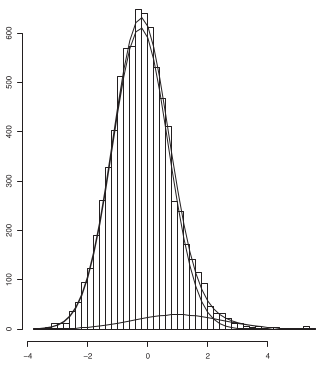
\includegraphics[width=.3\textwidth]{\figexp/MBB06-Bioinformatics-Fig3}
    \end{tabular}
  \end{tabular}
}

%====================================================================
\frame{\frametitle{Mixture model} 

  \begin{tabular}{cc}
    \hspace{-.04\textwidth}
    \begin{tabular}{p{.5\textwidth}}
      \paragraph{Easy EM.} Independent couples $(Z_i, Y_i)$
      $$
      p_\theta(Z_i \mid Y) = p_\theta(Z_i \mid Y_i)
      $$
      \ra Bayes formula:
      $$
      \widehat{\tau}_i = \Pbb_{\widehat{\theta}}\{Z_i = 1 \mid Y_i\}.
      $$
    \end{tabular}
    & 
    \hspace{-.02\textwidth}
    \begin{tabular}{p{.5\textwidth}}
    \paragraph{Graphical model:} ~\\  
      \includegraphics[width=.4\textwidth]{\figmhs/PolyMHS-GMmixture}
    \end{tabular}
  \end{tabular}
  
  \bigskip \bigskip \pause
  \paragraph{False discovery rate =} fraction of false positives among positives: 
  $$
  \widehat{FDR}(t) = \left. \sum_{i: \widehat{\tau}_i>t} (1 - \widehat{\tau}_i)  \right/ \#\{i: \widehat{\tau}_i>t\}. 
  $$
  \begin{itemize}
    \item Choose the detection threshold $t$ so that $\widehat{FDR}(t) \leq 5\%$ (say).
  \end{itemize}

}

%====================================================================
\frame{\frametitle{Semi-parametric mixture model} 

  \begin{tabular}{cc}
    \hspace{-.04\textwidth}
    \begin{tabular}{p{.5\textwidth}}
      \paragraph{Non-parametric emission distribution.} \nocite{RBD07,GRC09}
      \begin{itemize}
        \item Available prior estimate $\widehat{\pi}$ \refer{Sto02}
        \item Known null distribution
        $$
        p_\theta(Y_i \mid Z_i=0) = \Ncal(Y_i; 0, 1)
        $$
        \item Free alternative distribution 
      \end{itemize}
    \end{tabular}
    & 
    \hspace{-.1\textwidth}
    \begin{tabular}{p{.5\textwidth}}
      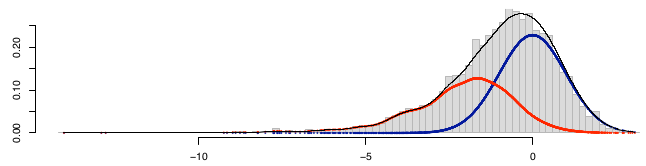
\includegraphics[width=.5\textwidth, trim=200 0 0 0, clip=]{\figfdr/GRC09-BMCBioinfo-Fig5a}
    \end{tabular}
  \end{tabular}
  
  \bigskip \bigskip \pause
  \paragraph{Kernel density estimate} of $f_1 = p_\theta(Y_i \mid Z_i=1)$:
  $$
  \widehat{f}_1(y) = \left. \sum_i \widehat{\tau}_i k(y - y_i) \right/ \sum_i \widehat{\tau}_i.
  $$
  
}

%====================================================================
\frame{\frametitle{Composed hypotheses} 

  \paragraph{More complex latent distribution.} $n$ genes, $Q$ comparison tests: 
  $$
  H_i^q = \{\text{gene $i$ is not differentially expressed in comparison $q$}\}
  $$
  \ra Latent variable: $Z_i = (Z_i^1, \dots Z_i^Q) \in \{0, 1\}^Q$, 
  $\Rightarrow 2^Q$ possible configurations.
  
  \bigskip \pause
  \begin{tabular}{cc}
    \hspace{-.04\textwidth}
    \begin{tabular}{p{.5\textwidth}}
      \paragraph{Mixture model.}
      \begin{itemize}
       \item $Z_i =$ gene configuration:
       $$p_\theta(Z) = p_\theta(Z_i^1, \dots Z_i^Q)$$
       \item $Y_i =$ probit $p$-values
       $$p_\theta(Y_i \mid Z_i) = \prod_q p_\theta(Y^q_i \mid Z_i^q)$$
       \pause
       \item Right: 5 time points.
       $$H^q = \{\Esp Y(t_{q-1}) = \Esp Y(t_q)\}.$$ 
       Genes with at least 2 successive differences.
      \end{itemize}
    \end{tabular}
    & 
    \hspace{-.02\textwidth}
    \begin{tabular}{c}
      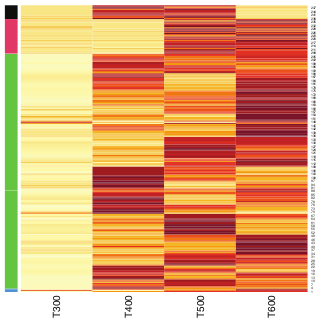
\includegraphics[width=.4\textwidth]{\figexp/MDM21-Bioinformatics-fig2} \\
      $Z =$ (\textcolor{black}{0110}), (\textcolor{red}{0011}), (\textcolor{green}{0111}), (\textcolor{blue}{1111})
    \end{tabular}
  \end{tabular}
  
}

%====================================================================
\frame{\frametitle{And also}

  \paragraph{Avatars of the Poisson distribution.} ~ \\
  \begin{itemize}
    \item Zero inflated Poisson = Mixture Dirac(0) + Poisson \\
    \ra Regular mixture \\ ~
    \item Over-dispersed Poisson = Negative binomial = Poisson-Gamma \\
    \ra Close form conditional distribution, thanks to conjugacy
  \end{itemize}

  \bigskip \bigskip \pause
  \paragraph{Gaussian mixed models.} ~ \\
  \begin{itemize}
    \item $Z =$ Gaussian random effect \\
    \ra Close form conditional distribution
  \end{itemize}

}

%====================================================================
%====================================================================
\section{More complex latent structure}
\frame{\frametitle{Outline} \tableofcontents[currentsection]}
%====================================================================
\frame{\frametitle{Copy number variation}

  \paragraph{Data.} $n$ locus along the genome, 
  $$
  Y_t = \text{noisy measurement of the number of copies at locus $t$}
  $$
  (should be two for diploids).
  
  \bigskip \pause
  \paragraph{Asumption.} 
  Neighbor loci often share the same number of copies.
  
  \bigskip \pause
  \paragraph{Example.} \refer{Hup08} 
  $$
  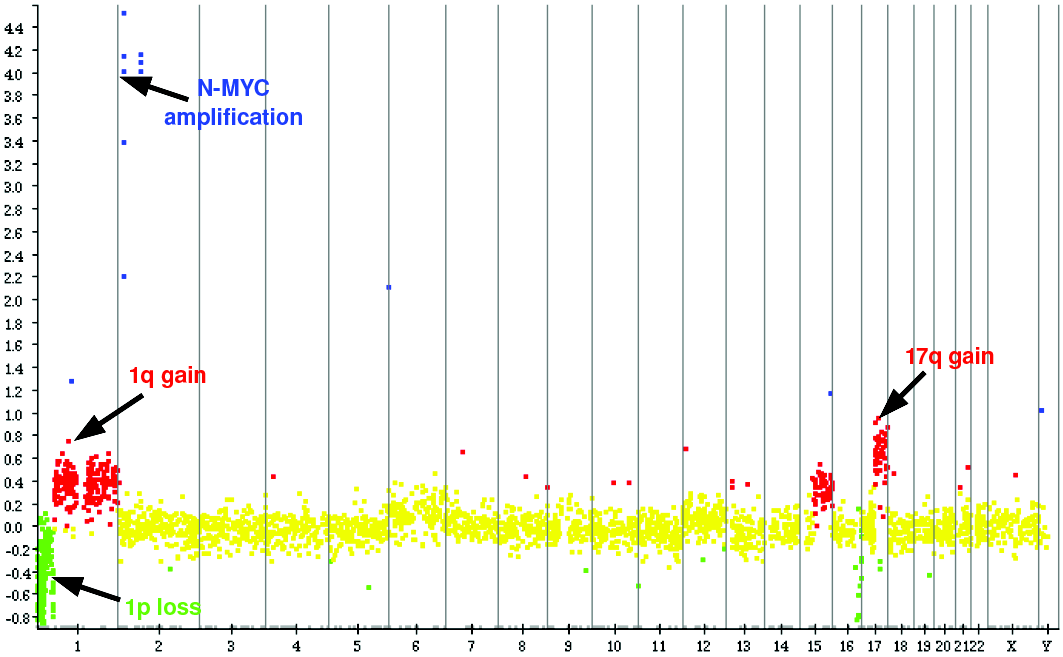
\includegraphics[width=.5\textwidth]{\figmhs/Hup08-Fig128a}
  $$

}

%====================================================================
\frame{\frametitle{Hidden Markov model}

  \paragraph{Latent variable model.} 
  \begin{itemize}
    \item $Z_t =$ status at locus $t$:
    $$
    Z = (Z_t)_{1 \leq t \leq n} \sim MC(\nu, \pi), 
    \qquad \text{($\nu=$ initial dist, $\pi =$ transition matrix)}
    $$
    \item $(Y_t)_{1 \leq t \leq n}$ independent $\mid Z$ : 
    $$
    (Y_t \mid Z_t = k) \sim \Ncal(\mu_k, \sigma^2).
    $$
    \item $\theta = (\nu, \pi, \mu, \sigma^2)$
    \item Graphical model:
    $$
    \includegraphics[width=.4\textwidth]{\figmhs/PolyMHS-GMhmm}
    $$
  \end{itemize}
  
  \bigskip \pause
  \paragraph{Inference.} E-step = forward-backward (= Baum-Welsh = Kalman = \dots) recursion.

  \bigskip \pause
  \paragraph{Classification.} Most probable hidden path $\widehat{Z}$  = Viterbi (dynamic programming) algorithm.

}

%====================================================================
\frame{\frametitle{Gene detection}

  \paragraph{Aim} starting from $Y =$ \\
  {\small
{\tt ATCTTTTTCGGCTTTTTTTAGTATCCACAGAGGTTATCGACAACATTTTCACATTACCAACCCCTGTGGACAAGGTTTTT} \\
{\tt TCAACAGGTTGTCCGCTTTGTGGATAAGATTGTGACAACCATTGCAAGCTCTCGTTTATTTTGGTATTATATTTGTGTTT} \\
{\tt TAACTCTTGATTACTAATCCTACCTTTCCTCTTTATCCACAAAGTGTGGATAAGTTGTGGATTGATTTCACACAGCTTGT} \\
{\tt GTAGAAGGTTGTCCACAAGTTGTGAAATTTGTCGAAAAGCTATTTATCTACTATATTATATGTTTTCAACATTTAATGTG} \\
{\tt TACGAATGGTAAGCGCCATTTGCTCTTTTTTTGTGTTCTATAACAGAGAAAGACGCCATTTTCTAAGAAAAGGAGGGACG} \\
{\tt \dots}
}

  \bigskip \bigskip 
  get
  $$
  \includegraphics[width=.9\textwidth]{\figgen/NBM02-NucAcidRes-Fig1}
  $$

}

%====================================================================
\frame{\frametitle{Modelling the Markov structure}

  \paragraph{Gene detection.} \refer{NBM02}
  \begin{itemize}
    \item $Y = (Y_t)_{1 \leq t \leq n}$ = (bacterial) genome ($n \sim 10^6$)
    \item $Z_t = $ coding status of nucleotide $t$
  \end{itemize}
  
  \bigskip \pause
  \paragraph{Transition graph of $(Z_t)$.} 
  $$
  \includegraphics[width=.7\textwidth]{\figmhs/genedetectionHMM_o6}
  $$

}

%====================================================================
\frame{\frametitle{Not modelling the emission distribution}

  \paragraph{Non-parametric HMM.} 
  Application of \refer{AMR09} to HMM
  \begin{itemize}
    \item HMM with non-parametric emission distributions are generically identifiable. \nocite{GCR16}
    \item No distribution assumptions (Gaussian, Poisson, Negative binomial, etc).
  \end{itemize}

  \bigskip \bigskip \pause
  \paragraph{Differentially expressed regions along the genome.} Kernel-density estimates in each of the $K=5$ states
  $$
  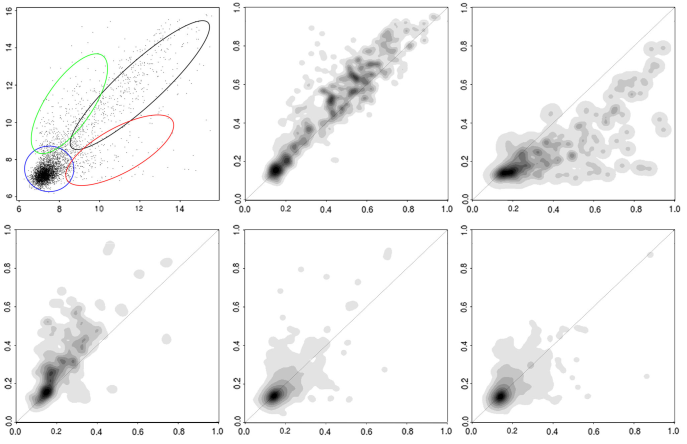
\includegraphics[width=.55\textwidth]{\figcp/GCR16-StatComp-Fig7}
  $$
}

%====================================================================
\frame{\frametitle{Tree-shaped Markov models}

  \paragraph{Remark.}
  The graphical model of an HMM is tree-shaped, likewise this of many evolutionary models.
  
  \bigskip \pause
  \begin{tabular}{cc}
    \hspace{-.04\textwidth}
    \begin{tabular}{p{.45\textwidth}}
      \paragraph{Phylogeny.}
      \begin{itemize}
       \item $Y =$ genomes of extant species
       \item $Z =$ ancestral genomes
      \end{itemize}
      
      \bigskip
      \paragraph{Likelihood for a given\footnote{Main problem in phylogeny = find the tree} tree\footnote{Breaks down for a network (e.g. horizontal transfert)}.} ~ \\
      Felsentein's algorithm \refer{Fel81} \\
      = 'upward-downward' recursion
      
    \end{tabular}
    & 
    \hspace{-.07\textwidth}
    \begin{tabular}{p{.5\textwidth}}
      \includegraphics[width=.45\textwidth]{\figmhs/PolyMHS-GMtree}
    \end{tabular}
  \end{tabular}

  
  \bigskip \pause
  \paragraph{Ancestral trait reconstruction.}
  Same problem and same solution for continuous (e.g. Brownian) latent $Z$ \refer{Lar14}. \nocite{BMR16}

}

%====================================================================
\frame{\frametitle{Other complex latent structures}

%   \paragraph{Non-parametric HMM.} 
%   \refer{AMR09} $\Rightarrow$ HMM with non-parametric emission distributions are generically identifiable. \nocite{GCR16}

  More complex latent structures may remain manageable using relevant algebraic properties. \\~
  \begin{itemize}
    \item Sequence partitioning (segmentation): dynamic programming \refer{AuL89}  and/or simple matrix products \\
    \ra quadratic complexity \nocite{RLR11} \\~
    \item Spanning tree\footnote{Phylogenetic trees are not spanning trees}-shaped graphical models: maximum spanning tree \refer{Kru56} and/or simple determinant calculation \refer{Cha82} \\
    \ra cubic complexity \nocite{SRS19} 
  \end{itemize}

  \bigskip
  \dots no generic rule to identify manageable E-steps.


}


%====================================================================
%====================================================================
\section{Too complex latent structure}
\frame{\frametitle{Outline} \tableofcontents[currentsection]}
%====================================================================
\frame{\frametitle{Interaction networks} 

  \paragraph{Data.} $Y = n \times n$ interaction matrix:
  $$
  Y_{ij} = 1 \text{ if entities $i$ and $j$ interact}, \quad = 0 \text{ otherwise}
  $$
  Entities = protein, genes, operons, \dots

  \bigskip
  \paragraph{Aim.} Cluster entities according to their interaction profile.
  
  \bigskip \pause
  \begin{tabular}{cc}
    \hspace{-.04\textwidth}
    \begin{tabular}{p{.5\textwidth}}
      \paragraph{Stochastic block-model.}
      \begin{itemize}
        \item $Z_i$ cluster membership of entity $i$
        $$
        \pi_i = \Pbb\{Z_i = k\}
        $$
        \item $Y_{ij}$ interaction $(i, j)$
        $$
        \gamma_{k\ell} = \Pbb\{Y_{ij} = 1 \mid Z_i = k, Z_j = \ell\}
        $$
        (can include covariates, strength, \dots).
      \end{itemize}
    \end{tabular}
    & 
    \hspace{-.02\textwidth}
    \begin{tabular}{p{.5\textwidth}}
      \includegraphics[width=.4\textwidth]{\figmhs/PolyMHS-GMsbm}
    \end{tabular}
  \end{tabular}
  
}

%====================================================================
\frame{\frametitle{Stochastic block-models} 

  \bigskip \pause
  \begin{tabular}{cc}
    \hspace{-.04\textwidth}
    \begin{tabular}{p{.5\textwidth}}
      \paragraph{Nasty conditional distribution.}
      \begin{itemize}
      \setlength\itemsep{1.25em}        
        \item 'Moralization' makes parents married
        \item The graphical model of $p_\theta(Z \mid Y)$ is a clique
        \item No nice factorization can be hoped to integrate it
        \item The E-step is intractable for, say, $n \geq 20$
      \end{itemize}
    \end{tabular}
    & 
    \hspace{-.02\textwidth}
    \begin{tabular}{p{.5\textwidth}}
      \includegraphics[width=.4\textwidth]{\figmhs/PolyMHS-GMsbmCond}
    \end{tabular}
  \end{tabular}
  
  \bigskip 
  \ra Regular EM does not apply

}

%====================================================================
\frame{\frametitle{Metabarcoding \& PLN model} 

  \paragraph{Data.} $n$ samples, $p$ species, 
  $$
  Y_{ij} = \text{\# of individuals (reads) from species $j$ in sample $i$}
  $$

  \bigskip \pause
  \begin{tabular}{cc}
    \hspace{-.04\textwidth}
    \begin{tabular}{p{.5\textwidth}}
      \paragraph{Poisson log-normal model.}
      \begin{itemize}
        \item Independent $(Z_i)_{1 \leq i \leq n}$: $Z_i \sim \Ncal_p(0, \Sigma)$, 
        \item Conditionally independent counts $(Y_{ij})$:
        $$
        (Y_{ij} \mid Z_{ij}) \sim \Pcal(\exp(Z_{ij}))
        $$
        (can include covariates, offset, ..)    
      \end{itemize}
    \end{tabular}
    & 
    \hspace{-.02\textwidth}
    \begin{tabular}{c}
    \includegraphics[width=.4\textwidth]{\figmhs/PolyMHS-GMmixture} \\
    $Y_i, Z_i \in \Rbb^p$
    \end{tabular}
  \end{tabular}

  \bigskip \pause
  \paragraph{Nasty conditional distribution.} $p_\theta(Z_i \mid Y_i) = p_\theta(Y_i, Z_i) / p_\theta(Y_i)$ but
  $$
  \text{no close form for} \quad p_\theta(Y_i) = \int p_\theta(Y_i, z_i) \d z_i
  $$
  \begin{itemize}
    \item Intractable E step
    \item Regular EM does not apply
  \end{itemize}
  
}

%====================================================================
\frame{\frametitle{Variational EM} 

  \paragraph{Principle.} Replace $p_\theta(Z \mid Y)$ with some approximation $q_\psi(Z)$
  \begin{itemize}
    \item $q_\psi$ chosen within a parametric distribution class $\Qcal$
    \item $\psi =$ variational parameter
  \end{itemize}
  
  \bigskip \pause
  \paragraph{Evidence lower bound (ELBO).}
  \begin{align*}
    ELBO(\theta, \psi) 
    & = \log p_\theta(Y) - KL(q_\psi(Z) || p_\theta(Z \mid Y)) \\
    & = \Esp_\psi[\log p_\theta(Y, Z)] - \Hcal(q_\psi)
  \end{align*}
    
  \bigskip \pause
  \paragraph{Variational EM.}
  \begin{align*}
    \psi^{h+1} 
    = \argmax_\psi ELBO(\theta^{(h)}, \psi)
    & = \argmin_\psi KL(q_\psi(Z) || p_{\theta^{(h)}}(Z \mid Y)), \\
    \theta^{(h+1)}
    = \argmax_\theta ELBO(\theta, \psi^{(h+1)})
    & = \argmax_\theta \Esp_{\psi^{(h+1)}}[\log p_\theta(Y, Z)]
  \end{align*}

}

%====================================================================
\frame{\frametitle{Variational EM} 

  \paragraph{Application.} Critical choice = choice of $\Qcal$
  \begin{description}
   \item[SBM:] $\Qcal =$ factorable distributions
   $$q_\psi(Z) = \prod_i q_{\psi_i}(Z_i)$$
   \item[PLN:] $\Qcal =$ Gaussian distributions
   $$q_{\psi_i}(Z_i) = \Ncal(Z_i; m_i, S_i)$$
  \end{description}

  \bigskip \bigskip \pause
  \paragraph{What do we know about VEM?}
  \begin{itemize}
    \item Computationally efficient
    \item Works well in practice (estimation, classification, \dots)
    \item Almost no theoretical guaranty
    \item Provides no measure of uncertainty
  \end{itemize}
  \ra Need to consider alternatives or post-processing
}

%====================================================================
\frame{\frametitle{Sequential Monte-Carlo for SBM} 

  \paragraph{Weighted SBM with covariates.} \nocite{DoR21}
  $$
  Y_{ij} \sim \Pcal(e^{\alpha_{k\ell} + x_i^\top \beta})
  $$
  VEM provides : an estimate $\widehat{\theta}_{VEM}$ and an approximate $q_\psi(Z)$.
  \\
  \ra Build an approximate posterior $p_{VEM}(Z, \theta \mid Y)$.

  \bigskip \bigskip \pause
  \paragraph{SMC algorithm.} Sample from a sequence of distributions
  $$
  p_h(Z, \theta \mid Y)
  \; \propto \;
  p(Z, \theta \mid Y)^{\emphase{\rho_h}} \; p_0(Z, \theta \mid Y)^{\emphase{1-\rho_h}}
  $$
  \begin{itemize}
    \item $p_0 =$ starting distribution ($p_{VEM}$, prior, \dots).
    \item $p_H =$ posterior, when $\rho_H = 1$, .
    \item $\rho_1, \dots, \rho_H$ tuned so to keep a sufficient effective sample size (ESS) at each step.
  \end{itemize}

}

%====================================================================
\frame{\frametitle{Sequential Monte-Carlo for SBM} 

  \paragraph{Choice of $p_0$.} Number of steps to reach the posterior \textcolor{cyan}{from $p_{VEM}$} or \textcolor{red}{from the prior}
  $$
  \includegraphics[width=.5\textwidth]{\figbayes/DoR21-Fig1-simu-rho} 
  $$
  (Synthetic data)
        
}

%====================================================================
\frame{\frametitle{An ecological example ($p = 51$ species)} 

  \begin{tabular}{cc}
    \hspace{-.04\textwidth}
    \begin{tabular}{p{.45\textwidth}}
      \paragraph{Posterior distribution for $\beta$:}
      \begin{itemize}
       \item \textcolor{orange}{$p_{VEM}$}
       \item \textcolor{darkgreen}{posterior with $\widehat{K}$} 
       \item \textcolor{pink}{(posterior with model averaging)}
      \end{itemize}
    \end{tabular}
    & 
    \hspace{-.1\textwidth}
    \begin{tabular}{c}
      \includegraphics[width=.25\textwidth]{\figbayes/DoR21-Fig7-beta1} 
      \includegraphics[width=.25\textwidth]{\figbayes/DoR21-Fig7-beta2}
    \end{tabular}
    \\ \pause
    ~ \\ ~\\
    \hspace{-.04\textwidth}
    \begin{tabular}{p{.45\textwidth}}
      \paragraph{Path to the posterior:}
      \begin{itemize}
       \item 25 steps to reach the posterior
       \item Mostly to recover the dependency structure between the $Z_i$
      \end{itemize}
    \end{tabular}
    & 
    \hspace{-.1\textwidth}
    \begin{tabular}{cc}
      $\rho_h$ & $MI(Z)$ \\
      \includegraphics[width=.25\textwidth, trim=0 0 0 30, clip=]{\figbayes/DoR21-Fig7-rho} &
      \includegraphics[width=.25\textwidth, trim=0 0 0 30, clip=]{\figbayes/DoR21-Fig7-MI}
    \end{tabular}
  \end{tabular}
      
}

%====================================================================
\frame{\frametitle{Monte-Carlo EM for PLN} 

  \paragraph{Monte-Carlo EM (MCEM).} Replace the E step with a sampling step
  \begin{align*}
  (Z^m)_{1 \leq m \leq M} \text{ iid} & \emphase{\sim p_{\theta}}(\cdot \mid Y) & 
  \to \quad
  \widehat{\Esp}[f(Z)] & = M^{-1} \sum_{m=1}^M f(Z^m).
  \end{align*}

  \bigskip \bigskip \pause
  \paragraph{Importance sampling.} When $p_{\theta}(Z \mid Y)$ not available, sample from a surrogate proposal:
  \begin{align*}
    (Z^m)_{1 \leq m \leq M} \text{ iid} & \emphase{\sim} q(\cdot) & 
    \to \quad \widehat{\Esp}[f(Z)] & = \sum_{m=1}^M w^m f(Z^m), \\
    \text{where} \quad w^m \propto \; p_{\theta}(Z^m \mid Y) & / q(Z^m).
  \end{align*}

  \bigskip \bigskip \pause
  \paragraph{Monte-Carlo EM.}
  \begin{itemize}
    \item Regular M step to update $\theta^{(h)}$,
    \item Monte-Carlo E step, using a Gaussian $q$ fitted to estimated the moments of $p_{\theta^{(h)}}(Z \mid Y)$,
    \item Starting with $q_\psi$ from VEM.
  \end{itemize}
}

%====================================================================
\frame{\frametitle{Composite likelihood} 

  \paragraph{Importance sampling} has poor efficiency (low ESS) in 'large' dimension ($p \geq 5, 10$).
  
  \bigskip \bigskip \pause
  \paragraph{Composite likelihood} = linear combination of marginal likelihoods:
  \begin{itemize}
    \item Spread the $p$ species into $B$ overlapping blocks $\Ccal_1, \dots \Ccal_B$ of size $k$;
    \item Define
    $$
    \cl_\theta(Y) = \sum_{b=1}^B \log p_\theta(Y^{\Ccal_b});
    $$
    \item Get $\widehat{\theta}_{\cl} = \argmax_\theta\cl_\theta(Y)$ using EM (which still applies);
    \item $\widehat{\theta}_{\cl}$ is asymptotically normal, with known asymptotic variance (Godambe information replaces Fisher information).
  \end{itemize}
  
  \bigskip \bigskip \pause
  \paragraph{MCEM for composite likelihood.} Same as before
  \begin{itemize}
    \item replacing the E step with e Monte Carlo step
    \item where importance sampling is made in dimension $k \ll p$.
  \end{itemize}

}

%====================================================================
%====================================================================
\section*{Conlusion}
\frame{\frametitle{Outline} \tableofcontents[currentsection]}
%====================================================================
\frame{\frametitle{Summary}

  \paragraph{Latent variable model =} generic and flexible modelling tool.
  
  \bigskip \bigskip 
  \paragraph{Inference} mostly depends on the complexity of the conditional distribution $p_\theta(Z \mid Y)$.
  
  \bigskip \bigskip \pause
  \paragraph{Variational approximations} provide efficient algorithms to manage too complex hidden structure, but with few statistical guaranties.
  
  \bigskip \bigskip 
  \paragraph{Monte Carlo-based} methods can take advantage of variational approximations, but at a computational cost.
  
}

%====================================================================
\frame{\frametitle{Some alternatives}

  \bigskip \bigskip 
  \paragraph{Classical MCMC-based} techniques often come at a prohibitive computational cost in genomics.

  \bigskip \bigskip \pause
  \paragraph{Variational auto-encoders} 
  \begin{itemize}
    \item provide more flexibility to fit the variational parameters ($\to$ better approximation)
    \item still relying on a Gaussian assumption
  \end{itemize}

  \bigskip \pause
  \begin{tabular}{cc}
    \hspace{-.04\textwidth}
    \begin{tabular}{p{.5\textwidth}}
      \paragraph{Learning some basic useful transforms.} ~\\
      'Learn' a smooth 1D transform 
      $$
      \psi = \psi_{\mu, \sigma^2, y},
      $$
      such that, if
      $$
      Z \sim \Ncal(\mu, \sigma^2)
      $$
      then
      $$
      \psi(Z) \sim p_{PLN(\mu, \sigma^2)}(Z \mid Y=y)
      $$
    \end{tabular}
    & 
    \hspace{-.02\textwidth}
    \begin{tabular}{c}
      $\mu = 0, \quad \sigma^2 = 1$ \\
      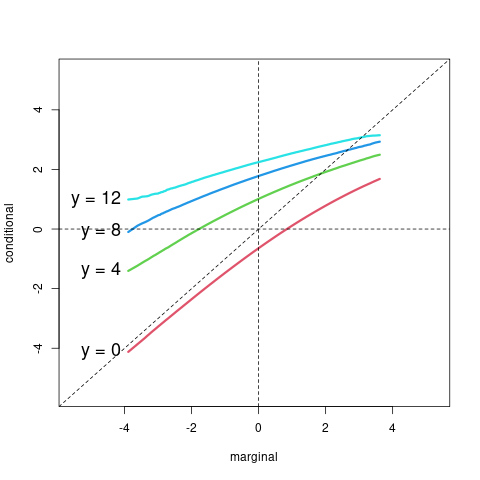
\includegraphics[width=.4\textwidth, trim=0 0 0 50, clip=]{\figeco/DirectSamplingPLNcondDist-transform}
    \end{tabular}
  \end{tabular}


}

%====================================================================
\frame[allowframebreaks]{ \frametitle{References}
  {
   \tiny
   \bibliography{BibGeneSMPGD}
   \bibliographystyle{alpha}
  }
}

%====================================================================
\backupbegin
%====================================================================

%====================================================================
\frame{\frametitle{Monte-Carlo EM for PLN} 

  $p$ species, blocks of size $k$

  $$
  \begin{tabular}{c|cc}
    \emphase{Log-likelihood $\log p_\theta(Y)$} & \multicolumn{2}{c}{\emphase{Composite log-likelihood  $\cl_\theta(Y)$}} \\    
    & & \\
    Synthetic data & \multicolumn{2}{c}{Barents fish ($n = 89$, $p=30$)} \\
    & & \\
    Normality & Estimates $\widehat{B}$ & ESS ($k=5$) \\
    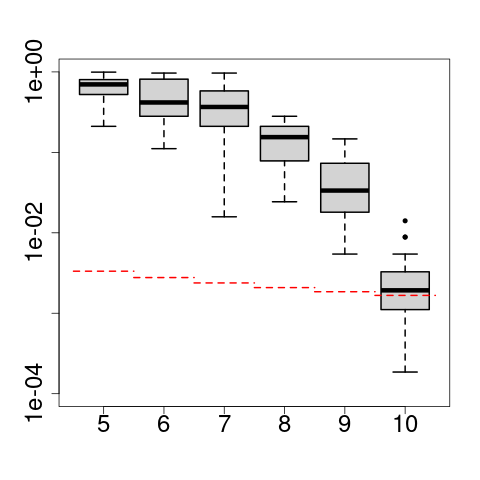
\includegraphics[width=.3\textwidth, trim=10 10 10 20, clip=]{\figbayes/StR24-Fig9} &
    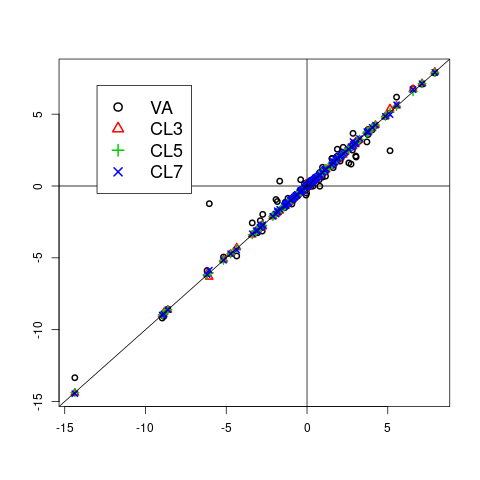
\includegraphics[width=.3\textwidth, trim=10 10 10 20, clip=]{\figbayes/StR24-Fig7a} &
    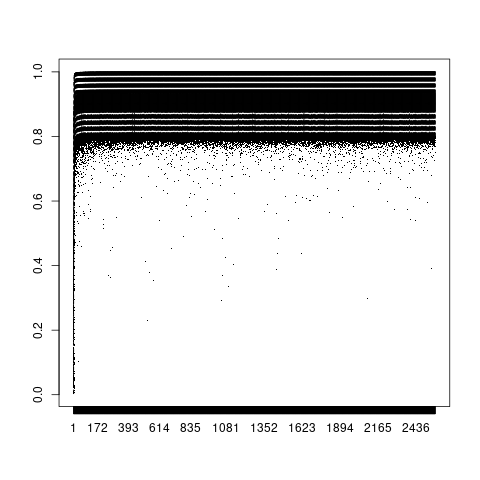
\includegraphics[width=.3\textwidth, trim=10 10 10 20, clip=]{\figbayes/StR24-Fig7c} \\    
    $KS$ p-val = f($p$) & Color = $k$ & $ESS =$ f(iteration)\\
  \end{tabular}
  $$

}

%====================================================================
\backupend
%====================================================================

%====================================================================
%====================================================================
\end{document}
%====================================================================
%====================================================================
  
  \begin{tabular}{cc}
    \hspace{-.04\textwidth}
    \begin{tabular}{p{.5\textwidth}}
    \end{tabular}
    & 
    \hspace{-.02\textwidth}
    \begin{tabular}{p{.5\textwidth}}
    \end{tabular}
  \end{tabular}

